\documentclass[8pt]{beamer}
\usepackage{tikz}
\usepackage[utf8]{vietnam}
\usepackage{amsmath}
\usepackage{graphicx}
\usepackage{wrapfig}
\usepackage{mathrsfs}
\usepackage{hyperref}
\usetheme{Copenhagen}
\usecolortheme{beaver}
\setbeamertemplate{navigation symbols}{}
\setbeamertemplate{headline}{}
\title[Chương 4: Biến đổi Laplace] %optional
{Chương 4: Biến đổi Laplace}
\subtitle{Tín hiệu và hệ thống}
\author[Tín hiệu và hệ thống] % (optional)
{Tín Vũ}
\date[VLC 2021] % (optional)
{tinvu1309@gmail.com}
\begin{document}
\frame{\titlepage}
\begin{frame}{Mục lục}
\tableofcontents
\end{frame}
\begin{frame}{Giới thiệu playlist}
\section{Giới thiệu playlist}
	\begin{itemize}
		\item Mình là Tín Vũ, hiện tại đang là sinh viên học tại Trường Đại học Công nghệ, Đại học Quốc gia Hà Nội. Mình tạo playlist video này để hỗ trợ các bạn học môn Tín hiệu và hệ thống trong các trường đại học kĩ thuật theo hướng \alert{trực quan hóa} nhất có thể.
		\item Do đó, mục tiêu của mình khi thực hiện playlist này không chỉ giúp các bạn ôn thi được điểm cao mà còn \alert{hiểu sâu công thức để làm nền tảng cho các môn học sau}.
		\item Để đạt được hai mục tiêu trên, các bạn nên xem \textbf{toàn bộ} video của mình, còn nếu chỉ cần ôn thi cấp tốc và đạt điểm cao thì hãy \textbf{bỏ qua} các video "optional".
		\item Nội dung playlist này chủ yếu bám sát nội dung môn học Tín hiệu và hệ thống tại trường của mình; nếu các bạn học trường khác, hãy tham khảo kĩ đề cương hay đề thi của trường bạn để đối chiếu sao cho ôn tập đúng trọng tâm và hợp lý. 
		\item Môn học này bao gồm \textbf{6} chương, các chương đều liên quan rất chặt chẽ và logic với nhau nên hãy học cẩn thận ngay từ \alert{chương 0} để ôn thi cuối kì đỡ vất vả.
	\end{itemize}
\end{frame}
\begin{frame}{Tài liệu tham khảo}
\section{Tài liệu tham khảo}
\begin{itemize}
		\item Tài liệu tham khảo chính: Signals and Systems (2nd edition) Alan V. Oppenheim and Alan S. Willsky.
		\item Tài liệu tham khảo phụ: Bài tập của mình học khóa trước, đề thi các năm cũ,...
		\item Tài liệu tham khảo phụ: Nếu bạn là sinh viên trường mình và muốn học "tủ" nhiều bài thì nên đọc Signals and Systems (2nd edition) Simon Haykin vì các thầy cô chủ yếu dạy và ra đề trong cuốn này, thế nhưng mình đánh giá cuốn này không đầy đủ và chi tiết như sách của Alan V. Oppenheim. 
	\end{itemize}
\end{frame}
\begin{frame}{Biến đổi Laplace}
\section{Khái niệm biến đổi Laplace}
\begin{itemize}
	\item Khái niệm biến đổi Laplace
\end{itemize}
Trong \alert{Chương 3}, chúng ta đã khảo sát rất kĩ bài toán chuỗi Fourier (CTFS) và biến đổi Fourier liên tục (CTFT) cho các tín hiệu \alert{\textbf{năng lượng}}. Ta rất dễ kiểm chứng với một vài dạng tín hiệu \alert{công suất} đơn giản, \alert{biến đổi Fourier không hội tụ}.
\\ Để "ép" tín hiệu công suất về dạng tín hiệu năng lượng sao cho có thể sử dụng được biến đổi Fourier, ta đặt một tham số phụ $s=\alert{\sigma}+j \omega$ và biến đổi như sau:
\begin{equation*}
\begin{split}
	X(s)&=\int_{-\infty}^{+\infty}x(t)e^{-st}dt=\int_{-\infty}^{+\infty}x(t)e^{-(\alert{\sigma}+j\omega)t}dt=\int_{-\infty}^{+\infty}x(t)e^{-j\omega t}\alert{e^{-\sigma t}}dt\\&=\mathscr{F}(x(t)\alert{e^{-\sigma t}})
\end{split}
\end{equation*}
Phần nhân tử $e^{-\alert{\sigma} t}$ có tác dụng "ép" $x(t)$ về dạng tín hiệu có năng lượng hữu hạn cơ bản, chúng ta mong muốn tìm tập giá trị của $\alert{\sigma=\Re(s)}$ sao cho $\mathscr{F}(x(t)\alert{e^{-\sigma t}})$ \textbf{tồn tại}.
\\ Ví dụ: tìm biến đổi Laplace và tập giá trị $\Re{(s)}$ sao cho biến đổi Fourier $\mathscr{F}(x(t)e^{-\sigma t})$ tồn tại.
$$x(t)=e^{t}u(t)$$
Ta có:
$$X(s)=\int_{-\infty}^{+\infty}x(t)e^{-st}dt=\int_{0}^{+\infty}e^{t}e^{-st}dt=\frac{e^{(1-s)t}}{1-s}\biggr|_{0}^{+\infty}=\frac{e^{(1-\sigma-j\omega)t}-1}{1-\sigma-j\omega}\biggr|^{+\infty}$$
Hiển nhiên $X(s)$ hội tụ khi và chỉ khi $1-\sigma<0$ ($e^{j\omega t}$ không liên quan do đây chỉ là thành phần điều hòa). Vậy ta tìm được \textbf{vùng hội tụ} (Region of convergence - ROC) của tín hiệu $x(t)$ là \alert{$\sigma>1$}, hay $\alert{\Re(s)>1}$.
\end{frame}
\begin{frame}{Biến đổi Laplace}

	Khi đó: $$X(s)=\frac{-1}{1-\sigma-j\omega}=\frac{1}{s-1} \quad \alert{(ROC:\Re{(s)}>1)}$$
Ta có thể minh họa kết quả này qua phác họa đơn giản sau:
\begin{figure}[h]
			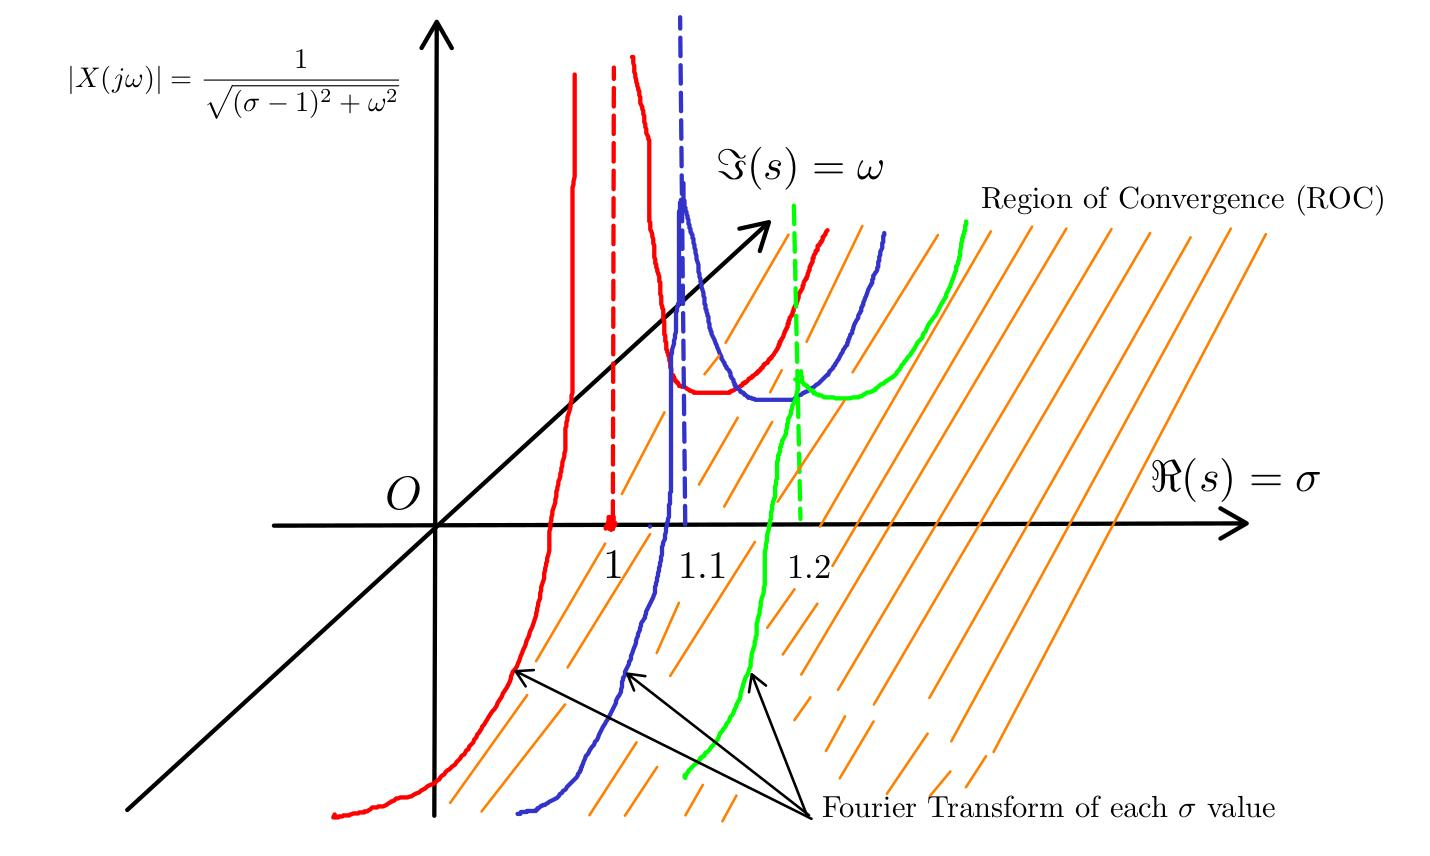
\includegraphics[width=0.9\textwidth]{laplace.jpg}
			\caption{Laplace Transform Visualization}\label{fig:re1}

		\end{figure}

\end{frame}
\begin{frame}{Biến đổi Laplace}
\section{Tính chất của biến đổi Laplace}
\begin{itemize}
	\item Tính chất của biến đổi Laplace
\end{itemize}
\begin{block}{Laplace transform pair}
If $x(t)$ is an arbitrary signal, we define Laplace transform formula:
$$X(s)=\int_{-\infty}^{+\infty}x(t)e^{-st}dt$$
$$x(t)=\frac{1}{2\pi j}\int_{\sigma-j\infty}^{\sigma+j\infty} X(s)e^{st}ds$$
\end{block}
Nếu các bạn đã học cẩn thận \alert{Chương 3} thì \alert{Chương 4} gần như hoàn toàn tương tự, điểm khác biệt duy nhất là \textbf{phải chỉ ra vùng hội tụ ROC trên s-plane}. Công thức (2) hoàn toàn không bao giờ được sử dụng trong môn học này, mà ta chỉ sử dụng công thức (1) kết hợp với bảng "Common Laplace transform pair" cùng với \textbf{phép toán tách phân thức} để biến đổi Laplace ngược.
\\ Ví dụ: tìm biến đổi Laplace của cặp tín hiệu (với $a>0$)
$$x_{1}(t)=e^{-at}u(t)$$ $$x_{2}(t)=-e^{-at}u(-t)$$ 
\end{frame}
\begin{frame}{Biến đổi Laplace}
Ta dùng trực tiếp công thức:
\begin{equation*}
\begin{split}
	X_{1}(s)&=\int_{-\infty}^{+\infty}x_{1}(t)e^{-st}dt=\int_{0}^{+\infty}e^{-at}e^{-st}dt=\frac{1}{s+a} \; \alert{(ROC: \Re{(s)}>-a)}\\
X_{2}(s)&=\int_{-\infty}^{+\infty}x_{2}(t)e^{-st}dt=-\int_{-\infty}^{0}e^{-at}e^{-st}dt=\frac{1}{s+a} \; \alert{(ROC: \Re{(s)}<-a)}
\end{split}
\end{equation*}
Vậy hiển nhiên ta thấy cùng một biến đổi trong miền s có thể cho ra 2 tín hiệu khác nhau trong miền thời gian \textbf{hoàn toàn phụ thuộc vào vùng ROC}.
\\ Ta định nghĩa phép toán $\mathscr{L}$ như sau:
\begin{equation*}
\begin{split}
	\mathscr{L}(x(t))&=X(s)\\
	\mathscr{L}^{-1}(X(s))&=x(t)
\end{split}
\end{equation*}
Từ phép toán trên cùng với định nghĩa hai tín hiệu $x(t)$, $y(t)$ có biến đổi Laplace:
\begin{equation*}
\begin{split}
	\mathscr{L}(x(t))&=X(s)\\
	\mathscr{L}^{-1}(X(s))&=x(t)
\end{split}
\end{equation*}
\begin{equation*}
\begin{split}
	\mathscr{L}(y(t))&=Y(s)\\
	\mathscr{L}^{-1}(Y(s))&=y(t)
\end{split}
\end{equation*}
\end{frame}
\begin{frame}{Biến đổi Laplace}

Ta liệt kê một vài tính chất quan trọng của biến đổi Laplace gồm:
\begin{enumerate}
	\item[1] Tính tuyến tính: $$\mathscr{L}(\alpha x(t)+\beta y(t))=\alpha\mathscr{L}(x(t))+\beta\mathscr{L}(y(t))$$
	\item[2] Dịch thời gian: $$\mathscr{L}(x(t-t_{0}))=X(s)e^{-jst_{0}}$$
	\item[3] Dịch trong miền s: $$\mathscr{L}(x(t)e^{s_{0}t})=X(s-s_{0})$$
	\item[4] Co giãn thời gian: $$\mathscr{L}(x(at))=\frac{1}{|a|}X\left(\frac{s}{a}\right)$$
	\item[5] Tích chập thời gian: $$\mathscr{L}(x(t)*y(t))=X(s)Y(s)$$
	\item[6] Đạo hàm miền thời gian: $$\mathscr{L}\left(\frac{dx(t)}{dt}\right)=sX(s)$$
	\item[7] Đạo hàm miền tần số: $$\mathscr{L}(-tx(t))=\frac{dX(s)}{ds}$$
	\item[8] Tích phân miền thời gian: $$\mathscr{L}\left(\int_{-\infty}^{t}x(\tau)d\tau\right)=\frac{X(s)}{s}$$
\end{enumerate}
\end{frame}
\begin{frame}{Biến đổi Laplace}
Suy ngẫm: chứng minh lại 8 tính chất trên. Gợi ý có thể tham khảo slide \alert{Chương 3}.
\\ Từ các tính chất trên ta cũng có bảng "Common Laplace Transform Pairs" như sau:
\begin{center}
\begin{tabular}{ |l|l| } 
 \hline
 $f(t)$ & $F(s)$ \\ 
 $\delta(t)$ & $1 \quad (ROC: \forall \Re{(s)})$ \\ 
 $u(t)$ &   $\frac{1}{s} \quad (ROC: \Re{(s)}>0)$ \\ 
 $-u(-t)$ & $\frac{1}{s} \quad (ROC: \Re{(s)}<0)$\\
 $e^{-at}u(t)$ & $\frac{1}{s+a}\quad (ROC: \Re(s)>-a)$\\
 $-e^{-at}u(-t)$ & $\frac{1}{s+a}\quad (ROC: \Re(s)<-a)$\\
 $e^{-at}\sin(\omega_{0}t)u(t)$ & $\frac{\omega_{0}}{(s+a)^2+\omega_{0}^2}\quad (ROC: \Re(s)>-a)$\\
 $e^{-at}\cos(\omega_{0}t)u(t)$ & $\frac{s+a}{(s+a)^2+\omega_{0}^2}\quad (ROC: \Re(s)>-a)$\\

 \hline
\end{tabular}
\end{center}
Suy ngẫm: sử dụng các tính chất biến đổi Laplace, hãy tự chứng minh lại toàn bộ bảng công thức này.
\\ Ví dụ: hãy xác định tín hiệu gốc $x(t)$ biết $ROC:-1<\Re{(s)}<2$
$$X(s)=\frac{s-1}{(s+1)(s-2)}$$
Ta không dùng trực tiếp công thức Laplace ngược mà thay vào đó ta sử dụng phương pháp \textbf{tách phân thức} và bảng trên:
\begin{equation*}
	X(s)=\frac{s-1}{(s+1)(s-2)}=\frac{A}{s+1}+\frac{B}{s-2}
\end{equation*}
\end{frame}
\begin{frame}{Biến đổi Laplace}
Đồng nhất hệ số, ta thu được:
$$X(s)=\frac{2}{3}.\frac{1}{s+1}+\frac{1}{3}.\frac{1}{s-2}$$
Quan sát vùng ROC được biểu diễn trên mặt phẳng s:
\begin{figure}[h]
			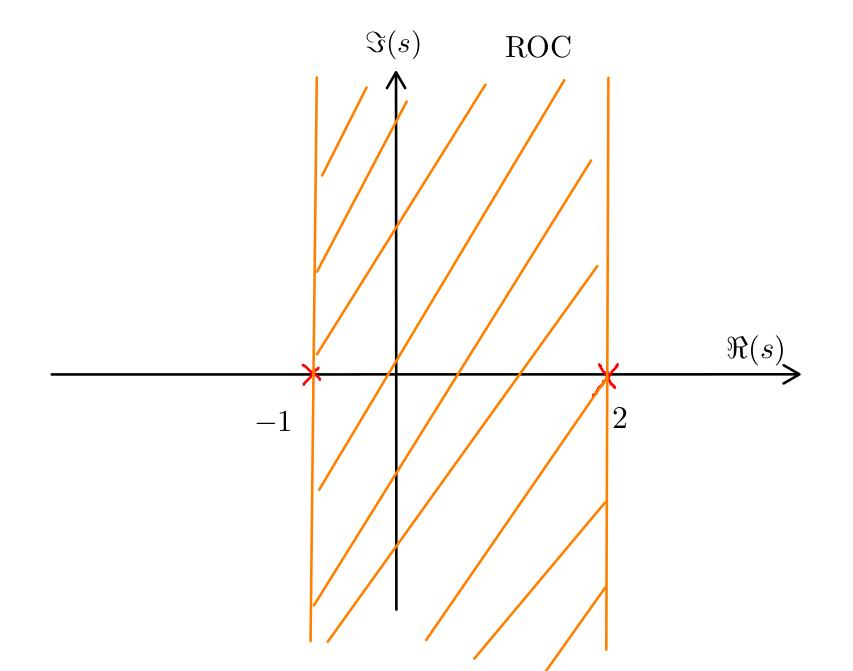
\includegraphics[width=0.3\textwidth]{roc.jpg}
			\caption{Region of convergence}\label{fig:re2}

		\end{figure}

Ta tra bảng và kết luận:
$$\mathscr{L}^{-1}\left(\frac{2}{3}.\frac{1}{s+1}+\frac{1}{3}.\frac{1}{s-2}\right)=\alert{\frac{2}{3}e^{-t}u(t)-\frac{1}{3}e^{2t}u(-t)}$$
Khi xét biển đổi Laplace ngược, ta phải \textbf{đặc biệt chú ý đến điều kiện vùng ROC của tín hiệu cũng như hệ thống}.
\end{frame}
\begin{frame}{Biến đổi Laplace}
\section{Phân tích hệ thống LTI liên tục}
\begin{itemize}
	\item Phân tích hệ thống LTI liên tục
\end{itemize}
\subsection{Phân tích tính chất của hệ thống}
\begin{itemize}
	\item[-] Phân tích tính chất của hệ thống
\end{itemize}
Xét một hệ thống có đáp ứng xung $h(t)$ với tín hiệu lối vào $x(t)$ và đáp ứng lối ra $y(t)$. Hiển nhiên từ tính chất tích chập đã phân tích ở trên, ta có:
$$y(t)=x(t)*h(t)\Rightarrow Y(s)=X(s)H(s) \Rightarrow \alert{H(s)=\frac{Y(s)}{X(s)}=\frac{(s-z_{1})(s-z_{2})\cdots}{(s-p_{1})(s-p_{2})\cdots}}$$
Ta gọi $H(s)$ là hàm truyền (transfer fucnction) của hệ thống. Sau khi biến đổi Laplace hàm truyền $H(s)$ luôn có thể được viết dưới dạng phân thức $H(s)=\frac{N(s)}{D(s)}$, ta định nghĩa hai khái niệm mới:
\begin{enumerate}
	\item \textbf{Điểm cực (poles)} của hệ thống: là tập nghiệm của phương trình $D(s)=0$
	\item \textbf{Điểm không (zeros)} của hệ thống: là tập nghiệm của phương trình $N(s)=0$
\end{enumerate}
Tính chất của hệ thống \alert{hoàn toàn phụ thuộc vào vị trí của các điểm cực và điểm không trên mặt phẳng s}.
\\Ví dụ: chỉ ra điểm cực và điểm không của hệ thống có hàm truyền $$H(s)=\frac{s^2+2s+3}{s^2+4}$$
Từ định nghĩa, ta giải phương trình $N(s)=0$ và $D(s)=0$, thu được các nghiệm cực và không như sau:
\begin{equation*}
\begin{cases}
z_{1,2}=-1\pm j\sqrt{2}\\
p_{1,2}=\pm 2j
\end{cases}
\end{equation*}
\end{frame}
\begin{frame}{Biến đổi Laplace}
Ta có thể rất dễ dàng biểu diễn các điểm cực và không trên mặt phẳng s
\begin{figure}[h]
			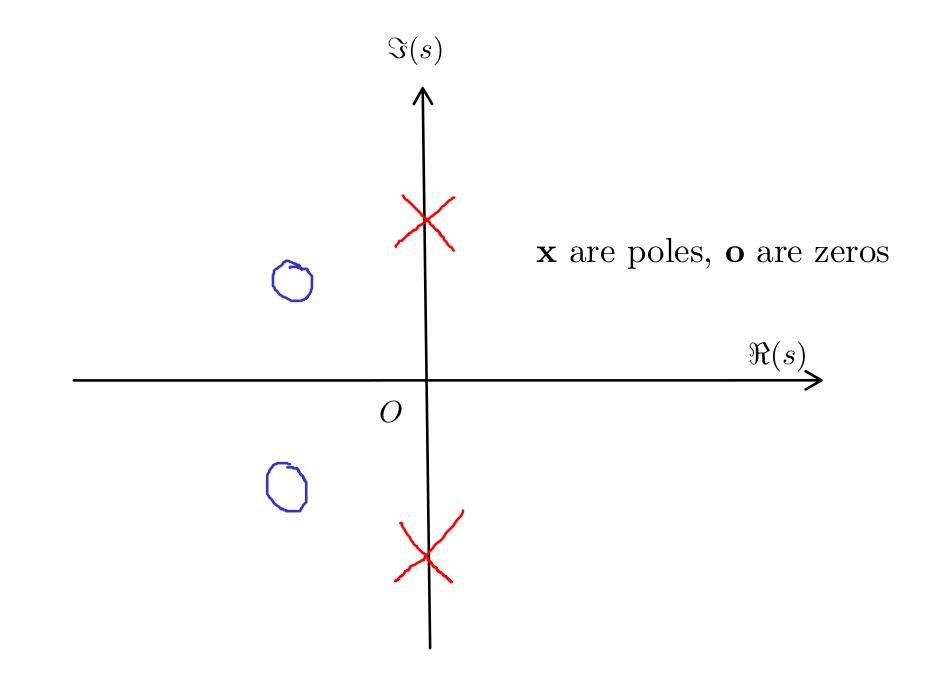
\includegraphics[width=0.6\textwidth]{zero.jpg}
			\caption{Representing zeros and poles in s-plane}\label{fig:re3}

		\end{figure}
		Khi xét đến tính chất đơn giản của hệ thống sử dụng biến đổi Laplace (trong giới hạn môn học này), ta chỉ xét đến \textbf{\alert{điểm cực}} của hệ thống mà thôi, tạm thời chưa cần quan tâm đến điểm không.
\end{frame}
\end{document}
